\documentclass{standalone}
\usepackage{tikz}
\usetikzlibrary{patterns, shadings}

\begin{document}
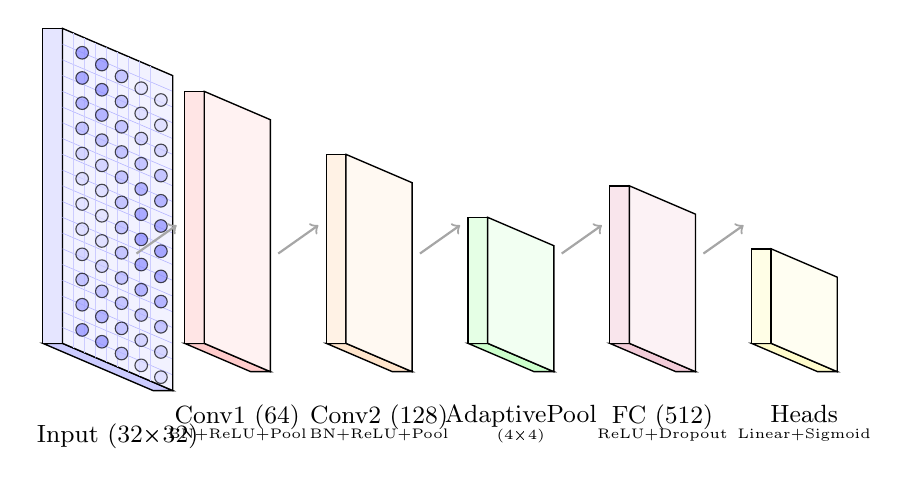
\begin{tikzpicture}[scale=1.0]
  % Define the perspective parameters
  \def\xshift{1.8}   % Horizontal shift between layers
  \def\yshift{0}     % Vertical shift
  \def\layerwidth{0.25}  % Width of each layer (thickness when viewed from side)
  \def\layerdepth{1.2}   % Depth of each layer

  % Input spectrogram - larger and more realistic
  \def\spectroheight{4.0}
  \def\spectrodepth{2.0}
  \begin{scope}[shift={(0,0)}]
    % Bottom face
    \filldraw[fill=blue!20, draw=black, line width=0.5pt]
      (0,0) -- (\layerwidth,0) --
      (\layerwidth+\spectrodepth*0.7,-\spectrodepth*0.3) --
      (\spectrodepth*0.7,-\spectrodepth*0.3) -- cycle;

    % Front face (spine)
    \filldraw[fill=blue!10, draw=black, line width=0.5pt]
      (0,0) -- (\layerwidth,0) -- (\layerwidth,\spectroheight) -- (0,\spectroheight) -- cycle;

    % Right side face (main spectrogram surface)
    \filldraw[fill=blue!5, draw=black, line width=0.5pt]
      (\layerwidth,0) -- (\layerwidth+\spectrodepth*0.7,-\spectrodepth*0.3) --
      (\layerwidth+\spectrodepth*0.7,\spectroheight-\spectrodepth*0.3) --
      (\layerwidth,\spectroheight) -- cycle;

    % Add realistic spectrogram pattern
    \begin{scope}
      \clip (\layerwidth,0) -- (\layerwidth+\spectrodepth*0.7,-\spectrodepth*0.3) --
            (\layerwidth+\spectrodepth*0.7,\spectroheight-\spectrodepth*0.3) --
            (\layerwidth,\spectroheight) -- cycle;

      % Frequency bins (horizontal lines)
      \foreach \y in {0.2,0.4,...,3.8} {
        \draw[blue!30, line width=0.2pt]
          (\layerwidth,\y) -- (\layerwidth+\spectrodepth*0.7,\y-\spectrodepth*0.3);
      }

      % Time frames (vertical lines)
      \foreach \t in {0.2,0.4,...,1.6} {
        \draw[blue!20, line width=0.2pt]
          (\layerwidth+\t*0.7,0-\t*0.3) -- (\layerwidth+\t*0.7,\spectroheight-\t*0.3);
      }

      % Spectral content (intensity patches)
      \foreach \i in {1,2,3,4,5,6} {
        \foreach \j in {1,2,...,12} {
          \pgfmathsetmacro{\intensity}{30+20*sin(\i*60)*cos(\j*30)}
          \filldraw[fill=blue!\intensity, opacity=0.7]
            (\layerwidth+\i*0.25,\j*0.32-\i*0.15) circle (0.08);
        }
      }
    \end{scope}

    % Label
    \node[below] at (\layerwidth+\spectrodepth*0.35,-\spectrodepth*0.3-0.3) {\small Input (32×32)};
  \end{scope}

  % Conv1 + BatchNorm + ReLU + MaxPool (64 channels)
  \def\conv1height{3.2}
  \begin{scope}[shift={(1*\xshift,0)}]
    \filldraw[fill=red!20, draw=black, line width=0.5pt]
      (0,0) -- (\layerwidth,0) --
      (\layerwidth+\layerdepth*0.7,-\layerdepth*0.3) --
      (\layerdepth*0.7,-\layerdepth*0.3) -- cycle;

    \filldraw[fill=red!10, draw=black, line width=0.5pt]
      (0,0) -- (\layerwidth,0) -- (\layerwidth,\conv1height) -- (0,\conv1height) -- cycle;

    \filldraw[fill=red!5, draw=black, line width=0.5pt]
      (\layerwidth,0) -- (\layerwidth+\layerdepth*0.7,-\layerdepth*0.3) --
      (\layerwidth+\layerdepth*0.7,\conv1height-\layerdepth*0.3) --
      (\layerwidth,\conv1height) -- cycle;

    \node[below] at (\layerwidth+\layerdepth*0.35,-\layerdepth*0.3-0.3) {\small Conv1 (64)};
    \node[below] at (\layerwidth+\layerdepth*0.35,-\layerdepth*0.3-0.6) {\tiny BN+ReLU+Pool};
  \end{scope}

  % Conv2 + BatchNorm + ReLU + MaxPool (128 channels)
  \def\conv2height{2.4}
  \begin{scope}[shift={(2*\xshift,0)}]
    \filldraw[fill=orange!20, draw=black, line width=0.5pt]
      (0,0) -- (\layerwidth,0) --
      (\layerwidth+\layerdepth*0.7,-\layerdepth*0.3) --
      (\layerdepth*0.7,-\layerdepth*0.3) -- cycle;

    \filldraw[fill=orange!10, draw=black, line width=0.5pt]
      (0,0) -- (\layerwidth,0) -- (\layerwidth,\conv2height) -- (0,\conv2height) -- cycle;

    \filldraw[fill=orange!5, draw=black, line width=0.5pt]
      (\layerwidth,0) -- (\layerwidth+\layerdepth*0.7,-\layerdepth*0.3) --
      (\layerwidth+\layerdepth*0.7,\conv2height-\layerdepth*0.3) --
      (\layerwidth,\conv2height) -- cycle;

    \node[below] at (\layerwidth+\layerdepth*0.35,-\layerdepth*0.3-0.3) {\small Conv2 (128)};
    \node[below] at (\layerwidth+\layerdepth*0.35,-\layerdepth*0.3-0.6) {\tiny BN+ReLU+Pool};
  \end{scope}

  % AdaptiveAvgPool
  \def\poolheight{1.6}
  \begin{scope}[shift={(3*\xshift,0)}]
    \filldraw[fill=green!20, draw=black, line width=0.5pt]
      (0,0) -- (\layerwidth,0) --
      (\layerwidth+\layerdepth*0.7,-\layerdepth*0.3) --
      (\layerdepth*0.7,-\layerdepth*0.3) -- cycle;

    \filldraw[fill=green!10, draw=black, line width=0.5pt]
      (0,0) -- (\layerwidth,0) -- (\layerwidth,\poolheight) -- (0,\poolheight) -- cycle;

    \filldraw[fill=green!5, draw=black, line width=0.5pt]
      (\layerwidth,0) -- (\layerwidth+\layerdepth*0.7,-\layerdepth*0.3) --
      (\layerwidth+\layerdepth*0.7,\poolheight-\layerdepth*0.3) --
      (\layerwidth,\poolheight) -- cycle;

    \node[below] at (\layerwidth+\layerdepth*0.35,-\layerdepth*0.3-0.3) {\small AdaptivePool};
    \node[below] at (\layerwidth+\layerdepth*0.35,-\layerdepth*0.3-0.6) {\tiny (4×4)};
  \end{scope}

  % Flatten + Linear (FC Hidden: 512)
  \def\fcheight{2.0}
  \begin{scope}[shift={(4*\xshift,0)}]
    \filldraw[fill=purple!20, draw=black, line width=0.5pt]
      (0,0) -- (\layerwidth,0) --
      (\layerwidth+\layerdepth*0.7,-\layerdepth*0.3) --
      (\layerdepth*0.7,-\layerdepth*0.3) -- cycle;

    \filldraw[fill=purple!10, draw=black, line width=0.5pt]
      (0,0) -- (\layerwidth,0) -- (\layerwidth,\fcheight) -- (0,\fcheight) -- cycle;

    \filldraw[fill=purple!5, draw=black, line width=0.5pt]
      (\layerwidth,0) -- (\layerwidth+\layerdepth*0.7,-\layerdepth*0.3) --
      (\layerwidth+\layerdepth*0.7,\fcheight-\layerdepth*0.3) --
      (\layerwidth,\fcheight) -- cycle;

    \node[below] at (\layerwidth+\layerdepth*0.35,-\layerdepth*0.3-0.3) {\small FC (512)};
    \node[below] at (\layerwidth+\layerdepth*0.35,-\layerdepth*0.3-0.6) {\tiny ReLU+Dropout};
  \end{scope}

  % Output heads (regression with sigmoid)
  \def\outheight{1.2}
  \begin{scope}[shift={(5*\xshift,0)}]
    \filldraw[fill=yellow!20, draw=black, line width=0.5pt]
      (0,0) -- (\layerwidth,0) --
      (\layerwidth+\layerdepth*0.7,-\layerdepth*0.3) --
      (\layerdepth*0.7,-\layerdepth*0.3) -- cycle;

    \filldraw[fill=yellow!10, draw=black, line width=0.5pt]
      (0,0) -- (\layerwidth,0) -- (\layerwidth,\outheight) -- (0,\outheight) -- cycle;

    \filldraw[fill=yellow!5, draw=black, line width=0.5pt]
      (\layerwidth,0) -- (\layerwidth+\layerdepth*0.7,-\layerdepth*0.3) --
      (\layerwidth+\layerdepth*0.7,\outheight-\layerdepth*0.3) --
      (\layerwidth,\outheight) -- cycle;

    \node[below] at (\layerwidth+\layerdepth*0.35,-\layerdepth*0.3-0.3) {\small Heads};
    \node[below] at (\layerwidth+\layerdepth*0.35,-\layerdepth*0.3-0.6) {\tiny Linear+Sigmoid};
  \end{scope}

  % Add arrows between layers
  \foreach \i in {0,1,2,3,4} {
    \pgfmathtruncatemacro{\nexti}{\i+1}
    \draw[->, thick, gray!70]
      (\i*\xshift+\layerwidth+\layerdepth*0.7+0.1, 1.5-\layerdepth*0.3) --
      (\nexti*\xshift-0.1, 1.5);
  }

\end{tikzpicture}
\end{document}
